\documentclass{beamer}

\usepackage[utf8]{inputenc}
\usepackage[T1]{fontenc}
\usepackage[spanish]{babel}
\usepackage{graphicx}
\usepackage{ragged2e}
\usepackage[table]{xcolor}
\usepackage{listings}
\usefonttheme[onlymath]{serif}

\definecolor{codegray}{rgb}{0.5,0.5,0.5}
\definecolor{backcolor}{rgb}{0.95,0.95,0.95}
\definecolor{verdecelda}{HTML}{B7CBA6}
\definecolor{rojocelda}{HTML}{FF9999}
\definecolor{lightgray}{gray}{0.6}


\usetheme{CambridgeUS}
\setbeamertemplate{navigation symbols}{}
\setbeamertemplate{blocks}[rounded][shadow=true]

\lstdefinestyle{mystyle}{
	backgroundcolor=\color{backcolor},
	commentstyle=\color{codegray},
	keywordstyle=\color{blue},
	numberstyle=\tiny\color{codegray},
	stringstyle=\color{red},
	basicstyle=\ttfamily\footnotesize,
	breaklines=true,
	captionpos=b,
	keepspaces=true,
	numbersep=5pt,
	showspaces=false,
	showstringspaces=false,
	showtabs=false,
	tabsize=2,
	inputencoding=utf8,
	extendedchars=true,
}

\lstset{style=mystyle}

\title{Trabajo Práctico 1}
\author{Cisnero, Seivane, Serafini}
\date{22 de Septiembre de 2025}

\begin{document}


\begin{frame}
	\centering
	
\includegraphics[width=0.25\textwidth]{UNAHUR (2)}
	\vfill
	{\huge \textbf{Trabajo Práctico 1}}\\[0.2cm]
	{\Large Aprendizaje Automático Avanzado}\\
	\vfill
	{\large Cisnero Matias, Seivane Nicolás, Serafini Franco}\\
	{\small 22 de Septiembre de 2025}
\end{frame}


\section{Ejercicio 1: Creación de Corpus}

\begin{frame}{}
	\centering
	\Large Ejercicio 1: Creación de Corpus\\
	\vspace{0.8cm}
	
\includegraphics[width=0.5\textwidth]{imagen_cortazar}
\end{frame}
	
\begin{frame}[fragile]{1.1 Descripción de Librerías Usadas}
	
	\justifying
	Se utilizaron las librerías de $r$ y $pdfplumber$, en la cual utilizamos la ultima para leer página por página de un pdf y la primera para seleccionar las palabras.\\
	\vspace{0.1cm}
	Los links a las librerías son los siguientes.\\
	\vspace{0.1cm}
	\href{https://pypi.org/project/pdfplumber/#extracting-text}{\textbf{pdfplumber}}\\
	\vspace{0.1cm}
	\href{https://docs.python.org/es/3.13/library/re.html}{\textbf{r}}
	\vspace{0.2cm}
	
\begin{block}{Funciones Utilizadas}
	\begin{columns}[c]
		\column{0.45\textwidth}
		\begin{itemize}
			\item \texttt{pdfplumber.open() as pdf}
			\item \texttt{pdf.pages[]}
			\item \texttt{.extract\_text()}
			\item \texttt{.split('\textbackslash n')}
		\end{itemize}
		
		\column{0.45\textwidth}
		\begin{itemize}
			\item \texttt{re.findall()}
			\item \texttt{.endswith()}
			\item \texttt{.strip()}
			\item \texttt{.isdigit()}
			\item \texttt{.split('\textbackslash n')}
		\end{itemize}
	\end{columns}
\end{block}
	
\end{frame}

		%pdfplumber.open() = se utiliza para ir a la dirección del pdf, retornando una instancia de la% clase $pdfplumber.PDF$ 
%$pdf.pages[]$ = es una propiedad de la clase $pdfplumber.PDF$, la cual se puede indexar para acceder a %las paginas del pdf representadas en la clase $pdfplumber.Page$
%$.extract_text()$ = Método de la clase $pdfplumber.Page$, recopila todos los objetos de caracteres de %la página en un sol string.
%$split('\_n')$ = Divide el string que se genero antes en los saltos de pagina, generando una lista de %lineas.
%$re.findall()$ =
%$.endswith()$ =
%$.strip()$ =
%$.isdigit()$ =

\begin{frame}[fragile]{1.2.1 Estructura de Código}
	
	\justifying
	\textbf{\underline{Se utiliza la siguiente estructura de codigo:}}\\
	\vspace{0.1cm}
	Se comienza importando las librerías y creando una lista de palabras, donde se irán agregando las extracciones de texto.
	\begin{lstlisting}[language=Python]
import pdfplumber
import re

words = []
	\end{lstlisting}
	\justifying
	En lo cual se sigue utilizando la función \texttt{pdfplumber.open() as pdf}, en la cual se debe especificar la ruta hacia el pdf. El cual nos devuelve $pdf$ como una instancia de la clase \texttt{pdfplumber.PDF}
		\begin{lstlisting}[language=Python]
with pdfplumber.open("ruta") as pdf:
	\end{lstlisting}
\end{frame}

	
\begin{frame}[fragile]{1.2.2 Estructura de Código}
	
	\justifying
	Se continua utilizando una propiedad de la clase \texttt{pdfplumber.Page}, de la cual se puede indexar para acceder a las paginas del pdf
	\begin{lstlisting}[language=Python]
with pdfplumber.open("ruta") as pdf:
	for page in pdf.pages[:]:
	\end{lstlisting}
	\justifying
	En lo cual se utiliza el metodo \texttt{.extract\_text()}, que recopila todos los objetos de caracteres de la página en un solo string.
	\begin{lstlisting}[language=Python]
with pdfplumber.open("ruta") as pdf:
	for page in pdf.pages[:]:
		text = page.extract_text()
		if text:
	\end{lstlisting}
\end{frame}
	
\begin{frame}[fragile]{1.2.3 Estructura de Código}
	
	\justifying
	Se continua diviendo el string segun el metodo \texttt{.split('\textbackslash n')}, el cual devuleve una lista de strings, los cuales fueron separados de acuerdo a \textbackslash n, ergo saltos de linea.
	\begin{lstlisting}[language=Python]
with pdfplumber.open("ruta") as pdf:
	for page in pdf.pages[:]:
		text = page.extract_text()
			if text:
				lines = text.split('\n')
	\end{lstlisting}
	\justifying
	Luego se sacan las lineas que sean numeros de pagina tanto en el pie de la misma como en el encabezado. La forma de extraccion varia de acuerdo a como es el pdf.
	\begin{lstlisting}[language=Python]
				if lines[-1].strip().isdigit():
					lines = lines[:-1]
				if lines[0].strip().isdigit():
					lines = lines[1:]
				
	\end{lstlisting}
\end{frame}
	
\begin{frame}[fragile]{1.2.4 Estructura de Código}
	
	\justifying
	Se crea por linea una lista con el método de la librería r:\\
	\vspace{0.1cm}
	\texttt{re.findall(r"\_w+|[.,!?;:]", line)}, en el cual se separan con expresiones regulares las palabras con \textbackslash w+ y aparte los signos de puntuación con [.,!?;:], en una lista de strings. Luego para cada palabra se la pasa a minúscula con el método \texttt{.lower()}.
	\begin{lstlisting}[language=Python]
with pdfplumber.open("ruta") as pdf:
	for page in pdf.pages[:]:
		text = page.extract_text()
		if text:
			lines = text.split('\n')
			if lines[-1].strip().isdigit():
				lines = lines[:-1]
			if lines[0].strip().isdigit():
				lines = lines[1:]
			for line in lines:
				tokens = re.findall(r"\w+|[.,!?;:]", line)
				tokens = [token.lower() for token in tokens]
	\end{lstlisting}

\end{frame}

	
\begin{frame}[fragile]{1.2.5 Estructura de Código}
	
	\justifying
	Luego se diferencia por linea los puntos aparte, los cuales consideeramos los ultimos puntos de las lineas. Cada linea, las cuales fueron convertidas en listas de strings son agregadas a la lista del corpus\\

	\begin{lstlisting}[language=Python]
with pdfplumber.open("ruta") as pdf:
	for page in pdf.pages[:]:
		text = page.extract_text()
			if text:
				lines = text.split('\n')
				if lines[-1].strip().isdigit():
					lines = lines[:-1]
				if lines[0].strip().isdigit():
					lines = lines[1:]
				for line in lines:
					tokens = re.findall(r"\_w+|[.,!?;:]", line)
					tokens = [token.lower() for token in tokens]
				if line.endswith("."):
					tokens[-1]= ". "
				words.extend(tokens)
	\end{lstlisting}
	
	
%%% RAYUELA LOCOOOO	
	
	
	
\end{frame}
	
\begin{frame}{1.3 Libros utilizados: Rayuela}
	\justifying
	\textbf{Titulo:} Rayuela\\
	\textbf{Autor:} Julio Cortazar\\
	\textbf{Año :} 1963\\
	Se extrayeron 197.342 caracteres y 20.810 caracteres únicos que conforman el vocabulario.\\
	\centering
	\vspace{0.2cm}
	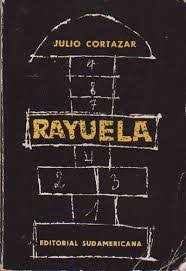
\includegraphics[width=0.3\textwidth]{rayuela_cortazar}
	
\end{frame}
	
\begin{frame}[fragile]{1.3.2 Código utilizado: Rayuela}
\begin{lstlisting}[language=Python]
with pdfplumber.open("Julio-Cortazar-Rayuela.pdf") as pdf:
	for page in pdf.pages[7:]:
		text = page.extract_text()
			if text:
				lines = text.split('\n')
				if lines[-1].strip().isdigit():
					lines = lines[:-1]
				if lines[0].strip().isdigit():
					lines = lines[1:]
				if lines[0].strip().isdigit():
					lines = lines[1:]
				if lines[-1].strip().isdigit():
					lines = lines[:-1]
				for line in lines:
					tokens = re.findall(r"\w+|[.,!?;:]", line)
					tokens = [token.lower() for token in tokens]
				if line.endswith("."):
					tokens[-1]= ". "
				words.extend(tokens)
\end{lstlisting}
	
\end{frame}
	
	
\begin{frame}{1.3.3 Ejemplo Borrado: Rayuela}
	\centering
	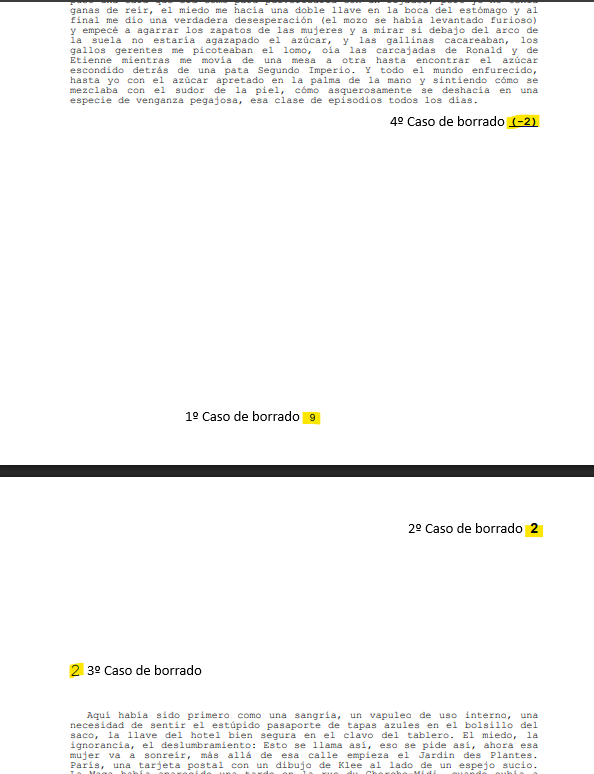
\includegraphics[width=0.5\textwidth]{borrado_rayuela}
	
\end{frame}	
	
	
%%% TODOS LOS FUEGOS

\begin{frame}{1.3 Libros utilizados: Todos los fuegos}
\justifying
\textbf{Titulo:} Todos los fuegos el fuego.\\
\textbf{Autor:} Julio Cortazar\\
\textbf{Año :} 1966\\
Se extrayeron 55.948 caracteres y 2.828 caracteres únicos que conforman el vocabulario.\\
\centering
\vspace{0.2cm}
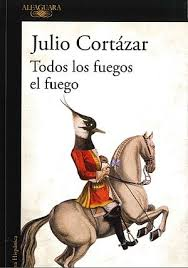
\includegraphics[width=0.3\textwidth]{todos_los_fuegos_cortazar}

\end{frame}

\begin{frame}[fragile]{1.3.2 Código utilizado: Todos los fuegos}
\begin{lstlisting}[language=Python]
with pdfplumber.open("Julio Cortazar Todos los fuegos.pdf") as pdf:
	for page in pdf.pages[:-1]:
		text = page.extract_text()
			if text:
				lines = text.split('\n')
				if lines[-1].strip().isdigit():
					lines = lines[:-1]
				for line in lines:
					tokens = re.findall(r"\w+|[.,!?;:]", line)
					tokens = [token.lower() for token in tokens]
				if line.endswith("."):
					tokens[-1]= ". "
				words.extend(tokens)
		\end{lstlisting}

\end{frame}


\begin{frame}{1.3.3 Ejemplo Borrado: Todos los fuegos}
\centering
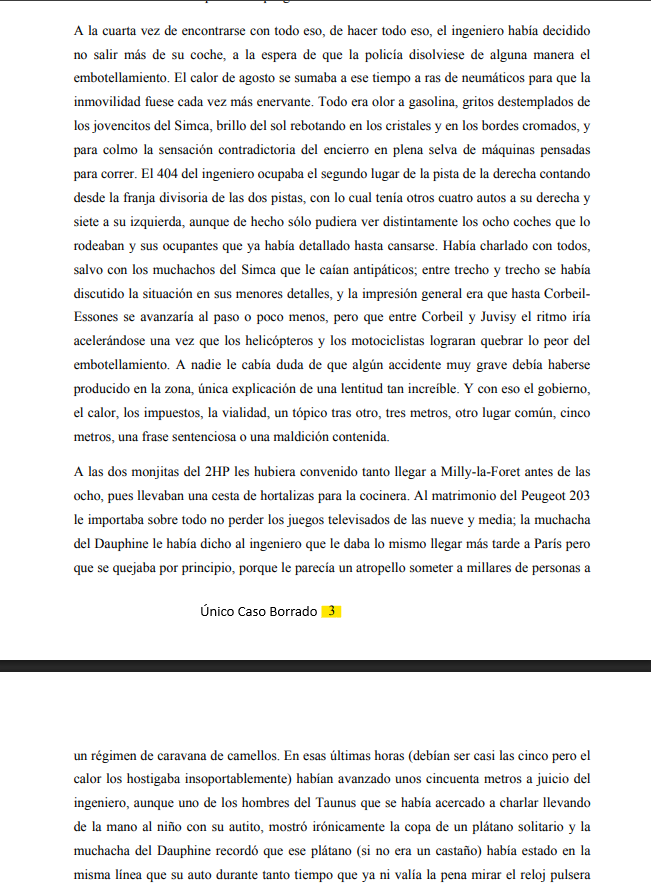
\includegraphics[width=0.5\textwidth]{borrado_todoslosfuegos}

\end{frame}	
	
%%% un tal lucas

\begin{frame}{1.3 Libros utilizados: Historias de cronopios y de famas}
	\justifying
	\textbf{Titulo:} Historias de cronopios y de famaso.\\
	\textbf{Autor:} Julio Cortazar\\
	\textbf{Año :} 1962\\
	Se extrayeron 32.224 caracteres y 2.514 caracteres únicos que conforman el vocabulario.\\
	\centering
	\vspace{0.2cm}
	
\includegraphics[width=0.3\textwidth]{historias_de_cronopios_y_de_famas_cortazar}
	
\end{frame}

\begin{frame}[fragile]{1.3.2 Código utilizado: Historias de cronopios y de famas}
	\justifying
	En este caso no fue necesario quitar ninguna linea.
	\begin{lstlisting}[language=Python]
with pdfplumber.open("Historias-de-Cronopios-y-de-Famas - Julio Cortazar.pdf") as pdf:
	for page in pdf.pages[3:-1]:
		text = page.extract_text()
			if text:
				lines = text.split('\n')
				for line in lines:
					tokens = re.findall(r"\w+|[.,!?;:]", line)
					tokens = [token.lower() for token in tokens]
				if line.endswith("."):
					tokens[-1]= ". "
				words.extend(tokens)
	\end{lstlisting}
	
\end{frame}
	
	
%% ahora si un tal lucas

\begin{frame}{1.3 Libros utilizados: Un tal Lucas.}
	\justifying
	\textbf{Titulo:} Un tal Lucas.\\
	\textbf{Autor:} Julio Cortazar\\
	\textbf{Año :} 1979\\
	Se extrayeron 32.224 caracteres y 2.514 caracteres únicos que conforman el vocabulario.\\
	\centering
	\vspace{0.2cm}
	
\includegraphics[width=0.3\textwidth]{un_tal_lucas_cortazar}
	
\end{frame}

\begin{frame}[fragile]{1.3.2 Código utilizado: Un tal Lucas.}
	\begin{lstlisting}[language=Python]

with pdfplumber.open("Lucas_Julio_Cortazar.pdf") as pdf:
	for page in pdf.pages[5:]:
		text = page.extract_text()
			if text:
				lines = text.split('\n')
				if lines[-1].strip().isdigit():
					lines = lines[:-1]
				lines = lines[1:]
				for line in lines:
					tokens = re.findall(r"\w+|[.,!?;:]", line)
					tokens = [token.lower() for token in tokens]
				if line.endswith("."):
					tokens[-1]= ". "
				words.extend(tokens)
	\end{lstlisting}
	
\end{frame}


\begin{frame}{1.3.3 Ejemplo Borrado: Un tal Lucas.}
	\centering
	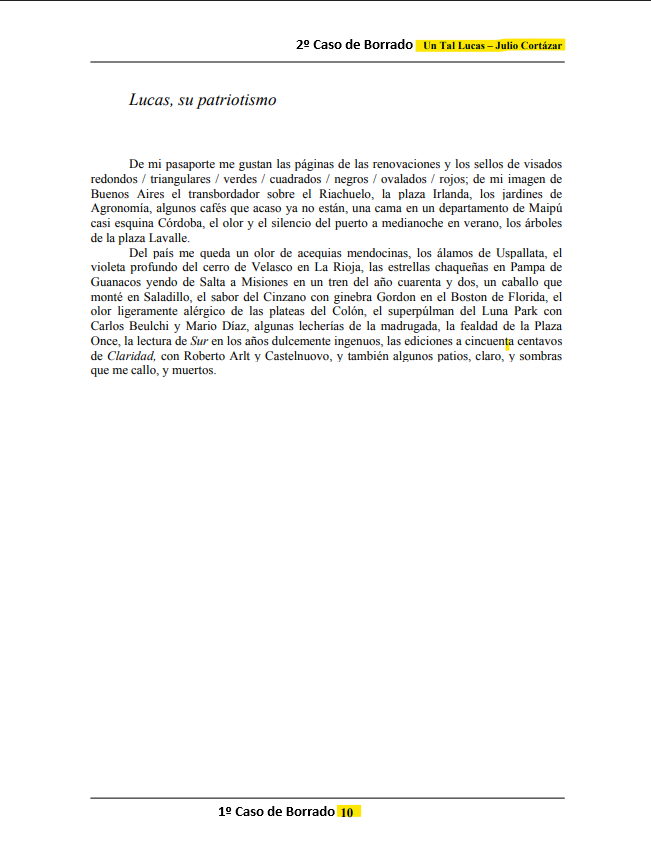
\includegraphics[width=0.5\textwidth]{borrado_un_tal_lucas}
\end{frame}	
	
	
\begin{frame}[fragile]{1.4 Corpus final}
	\justifying
	Se guarda el corpus final en un archivo llamado \textbf{corpus.txt}.
	
	\begin{lstlisting}[language=Python]
		with open("corpus.txt", "w", encoding="utf-8") as f:
			f.write("\n".join(words))
	\end{lstlisting}
	
	Obteniendo un corpus como se ve en la siguiente imagen.
	\vspace{0.1cm}
\begin{columns}[t] % [t] para alinear arriba
	\column{0.55\textwidth}
	\textbf{Vocabulario (único):} 27.971\\
	\textbf{Corpus total:} 310.347
	
	\column{0.45\textwidth}
	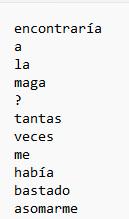
\includegraphics[width=0.5\linewidth]{corpus_txt.png}
\end{columns}

\end{frame}


\section{Ejercicio 2: Implementación CBOW y SkipGram}

\begin{frame}{}
	\centering
	\Large Ejercicio 2: Implementación CBOW y SkipGram\\
	\vspace{0.8cm}
	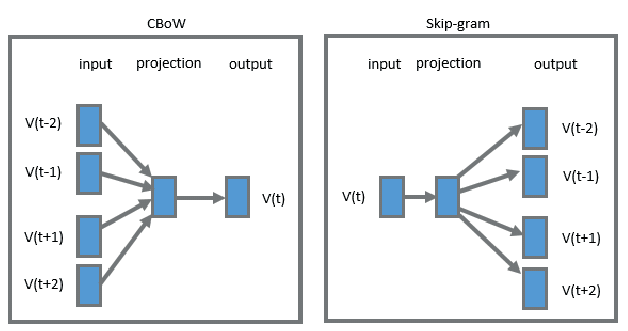
\includegraphics[width=0.5\textwidth]{imagenes_cbow_skipgram}
\end{frame}



	
\begin{frame}[fragile]{2.1 Pasos previos}
	\justifying
	Se abre y carga el \textbf{corpus.txt}.
	
	\begin{lstlisting}[language=Python]
with open("corpus.txt", "r", encoding="utf-8") as f:
	corpus = f.read().splitlines()
	\end{lstlisting}
	Luego se crean los diccionarios que se utilizaran en ambos métodos.
	\begin{lstlisting}[language=Python]
    vocab = sorted(set(corpus))
		vocab_tamano = len(vocab)
		palabra_a_indice = {palabra: i for i, palabra in enumerate(vocab)}
		indice_a_palabra = {i: palabra for i, palabra in enumerate(vocab)}
	\end{lstlisting}

\end{frame}
	
\section{Ejercicio 2. A:CBOW}
	
\begin{frame}[fragile]{2.2 CBOW}
	\begin{block}{\textbf{Definición:} Continuous Bag of Words(CBOW)}
	\justifying
	\vspace{0.1cm}
	\textbf{Propósito:} Es un modelo de aprendizaje automático para aprender representaciones de palabras que capturan el "significado" de las palabras basadas en su contexto.\\
	\vspace{0.1cm}
	\textbf{Principio:} A diferencia de los modelos más simples, CBOW utiliza un contexto de $C$ palabras para predecir una palabra central\\
	\vspace{0.1cm}
	\textbf{Contexto vs. Predicción:}  A partir de un contexto de $C$ palabras ($p_{I,1}, p_{I,2}, ..., p_{I,C}$), se intenta predecir la palabra objetivo ($p_O$), que generalmente es la palabra central
\end{block}
	
\end{frame}
	
	
\begin{frame}[fragile]{2.2 CBOW: Conceptos Fundamentales}
	\begin{block}{\textbf{Definición:} Continuous Bag of Words(CBOW)}
		\justifying
		\vspace{0.1cm}
		\textbf{Propósito:} El objetivo es encontrar representaciones vectoriales ($v_p$) para cada palabra en el vocabulario $V$. Estas representaciones se optimizan para que las palabras que comparten contextos sean más similares (tengan un producto interno alto)\\
		\vspace{0.1cm}
		\textbf{Principio:} A diferencia de los modelos más simples, CBOW utiliza un contexto de $C$ palabras para predecir una palabra central\\
		\vspace{0.1cm}
		\textbf{Contexto vs. Predicción:}  A partir de un contexto de $C$ palabras ($p_{I,1}, p_{I,2}, ..., p_{I,C}$), se intenta predecir la palabra objetivo ($p_O$), que generalmente es la palabra central
	\end{block}
	
\end{frame}

\begin{frame}[fragile]{2.2 CBOW: Arquitectura del Perceptrón}
	\begin{block}{\textbf{Arquitectura}}
		\justifying
		\vspace{0.1cm}
		\textbf{Estructura:} El calculo se enmarca en un \textbf{perceptron multicapa}\\
		\vspace{0.1cm}
		\textbf{Entrada:} Se presentan las $C$ palabras de contexto. La representación de las entradas se realiza mediante la \textbf{codificación One-hot}\\
		\vspace{0.1cm}
		\textbf{Diccionario ($V$):} Las palabras pertenecen a un diccionario $V$ cuyo cardinal es $|V|$ \\
		\vspace{0.1cm}
		\textbf{Capa Oculta:} Tiene una única capa oculta con $N$ unidades, todas con función de activación lineal $g(x) = x$ \\
		\vspace{0.1cm}
		\textbf{Dimensiones de Pesos:} 						\\
		\begin{itemize}
			\item Matriz de pesos Entrada-Oculta ($W$): $W \in |V| \times N$\\
			\item Matriz de pesos Oculta-Salida ($W'$): $W' \in N \times |V|$
		\end{itemize}
		\vspace{0.1cm}
		\textbf{Salida:} La función de activación de las unidades de salida es soft-max 
	\end{block}
	
\end{frame}
	
	
\begin{frame}[fragile]{2.2 CBOW: Arquitectura del Perceptrón}
\centering
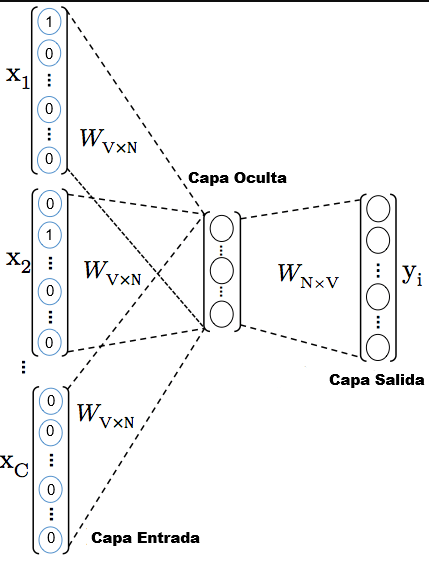
\includegraphics[width=0.45\textwidth]{CBOW_arquitectura}
	
\end{frame}


\begin{frame}[fragile]{2.2 Calculo de representación Contextual (h)}

		\justifying
		\textbf{Cálculo de $h$:} Se $h$ calcula como el \textbf{promedio de las filas} de $W$ que corresponden a los índices de las palabras en el contexto\\
		\vspace{0.1cm}
		\textbf{Representaciones One-Hot:}  Sea $x_1, x_2, ..., x_C$ las representaciones one-hot de las $C$ palabras en el contexto\\
		\vspace{0.1cm}
		\textbf{Representaciones Contextuales ($v_p$):} Sea $v_{p_i}$ la representación contextual de la palabra $p_i$ (que es la fila $i$ de $W$ donde $i$ es el índice de $p_i$ en $V$) \\
		\vspace{0.1cm}
		\textbf{Fórmula de $h$:} 						\\
		\begin{itemize}
			\item Cálculo del vector $h$: 	
			$$h = \frac{1}{C} W^t(x_1 + x_2 + \dots + x_C)$$\\
			\item Cálculo de $h$ usando $v_p$:
			 $$h = \frac{1}{C} (v_{p1} + v_{p2} + \dots + v_{pC})$$
		\end{itemize}
	\begin{lstlisting}[language=Python]
		with open("corpus.txt", "r", encoding="utf-8") as f:
		corpus = f.read().splitlines()
	\end{lstlisting}
	Luego se crean los diccionarios que se utilizaran en ambos métodos.
	\begin{lstlisting}[language=Python]
		vocab = sorted(set(corpus))
		vocab_tamano = len(vocab)
		palabra_a_indice = {palabra: i for i, palabra in enumerate(vocab)}
		indice_a_palabra = {i: palabra for i, palabra in enumerate(vocab)}
	\end{lstlisting}
	
\end{frame}

	
\begin{frame}[fragile]{2.2 Calculo de representación Contextual (h)}

	\begin{lstlisting}[language=Python]
		h = cp.mean(W[indices_contextos], axis=0).reshape(-1,1)
	\end{lstlisting}
	Donde se utiliza la función \texttt{cupy.mean(a, axis=None, dtype=None, out=None, keepdims=False)}, que retorna la media de la matriz de entrada $a$ a lo largo del eje. 
	
	\begin{block}{Explicación}
	\begin{itemize}
	\item W[indices$\_$contextos] selecciona los vectores de embedding correspondientes a esas palabras\\
	\item axis=0 significa promediar columna por columna.
	\[
	h = \frac{1}{C} \sum_{i=1}^{C} v_{p_i}
	= \left(
	\frac{1}{C}\sum_{i=1}^C w_{i1}, \;
	\frac{1}{C}\sum_{i=1}^C w_{i2}, \;
	\dots, \;
	\frac{1}{C}\sum_{i=1}^C w_{id}
	\right)
	\]
\end{itemize}
	\end{block}
\end{frame}



\begin{frame}[fragile]{2.2 Salida de la Red}
	\begin{block}{Excitación de la salida}
\justifying
\textbf{ Vector de Salida ($v'_{p_j}$):} La columna $j$ de la matriz $W'$ se denota como $v'_{p_j}$, siendo el vector de salida para la palabra $p_j$\\
\vspace{0.3cm}
\textbf{Estado de Excitación ($u_j$)} El estado de excitación de cada unidad de salida $j$ ($u_j$) se calcula como el producto interno del vector de salida $v'_{p_j}$ y la activación de la capa oculta $h$\\
$$u_j = (\mathbf{v}'_{p_j})^t \mathbf{h} \quad$$
Siendo en el código
\begin{lstlisting}[language=Python]
	u = W_prima.T@h
\end{lstlisting}
	\end{block}
\end{frame}
	
	
\begin{frame}[fragile]{2.2 Salida de la Red (Softmax)}
	\begin{block}{Excitación de la salida}
		\justifying
		\textbf{ Activación de Salida ($y_j$):} La función de activación de las unidades de salida es soft-max. El estado de activación $y_j$ de la unidad $j$ se calcula de la siguiente manera\\
		$$y_j = \frac{\exp u_j}{\sum_{j'=1}^{|V|} \exp u_{j'}} \quad$$
		\vspace{0.3cm}
		\textbf{ Interpretación:} El valor de $y_j$ se interpreta como la probabilidad de que la palabra objetivo sea $p_j$ dado el contexto que entra a la red ($p_{I,1}, \dots, p_{I,C}$)\\
		$$P(p_j/p_{I,1}, \dots, p_{I,C}) = y_j \quad$$
		Siendo en el código
		\begin{lstlisting}[language=Python]
			y = softmax(u)
		\end{lstlisting}
		Donde 
				\begin{lstlisting}[language=Python]
		def softmax(u):
			u_max = np.max(u)
			e_u = np.exp(u - u_max)
			return e_u / e_u.sum()
		\end{lstlisting}
	\end{block}
\end{frame}
	
	
\begin{frame}[fragile]{2.2 Salida de la Red (Softmax)}
	\begin{block}{Excitación de la salida}
		\justifying
		Siendo en el código
		\begin{lstlisting}[language=Python]
			def softmax(u):
			u_max = np.max(u)
			e_u = np.exp(u - u_max)
			return e_u / e_u.sum()
		\end{lstlisting}
		\textbf{ Consideraciones:} Se le resta a $u$ el maximo de $u$, ya que generaba errores $nan$ en los pesos\\
		\vspace{0.2cm}
		\textbf{ Explicación:} Restar $u\_max$ evita problemas numéricos por exponentes grandes, llamado overflow\\
		\[
		\frac{e^{u_i - c}}{\sum_j e^{u_j - c}} 
		= \frac{e^{u_i} e^{-c}}{\sum_j e^{u_j} e^{-c}} 
		= \frac{e^{u_i}}{\sum_j e^{u_j}}
		\]

	\end{block}
\end{frame}
	
	
\begin{frame}[fragile]{2.2 Función de Pérdida ($E$)}
	\begin{block}{}
		\justifying
		\textbf{Objetivo:} Minimizar la función de pérdida $E$, que es el negativo del logaritmo de la probabilidad de la palabra objetivo $p_O$ dado el contexto ($p_{I,1}, \dots, p_{I,C}$).\\[0.2cm]
		
		\textbf{Pérdida Logarítmica:} 
		\[
		E = - \log p(p_O \mid p_{I,1}, p_{I,2}, \dots, p_{I,C})
		\] \\[0.1cm]
		
		\textbf{Error ($e_j$):} Se define como la diferencia entre la predicción y el objetivo:
		\[
		e_j = y_j - t_j
		\]
		donde
		\[
		t_j =
		\begin{cases}
			1 & \text{si } j = j^* \text{ (índice de la palabra objetivo $p_O$)}\\
			0 & \text{si } j \neq j^*
		\end{cases}
		\] \\[0.1cm]
	\end{block}

\end{frame}
	
\begin{frame}[fragile]{2.2 Función de Pérdida y Derivada}
	\begin{block}{Función de Pérdida}
		La función de pérdida se define como:
\[
\begin{aligned}
	E &= - \log p(p_O \mid p_{I,1}, p_{I,2}, \dots, p_{I,C}) \\
	&= - u_{j^*} + \log \sum_{j'=1}^{|V|} \exp u_{j'} \\
\end{aligned}
\]
		\textbf{Derivada del error respecto al estado de excitación $u_j$:}
		\[
		\frac{\partial E}{\partial u_j} = y_j - t_j = e_j
		\]
			En código es
		\begin{lstlisting}[language=Python]
			e = y
			e[indice_central] -= 1
		\end{lstlisting}

	\end{block}
\end{frame}
	
\begin{frame}[fragile]{2.2 Actualización de $W'$ (Pesos Oculta-Salida)}
	\begin{block}{Actualización de pesos}
	La regla de actualización para $W'$ en CBOW es idéntica a la del contexto de una sola palabra, ya que solo se modificó el cálculo de $h$\\
	Derivando $E$ respecto a $w'_{ij}$ obtenemos la regla de actualización:\\
	En forma vectorial:
	\[
	W'_{\cdot,j}(\text{nuevo}) = W'_{\cdot,j}(\text{anterior}) - \eta \, e_j \, h
	\]
	Considerando las columnas de $W'$ como vectores de salida $v'_j$:
	\[
	v'_j(\text{nuevo}) = v'_j(\text{anterior}) - \eta \, e_j \, h
	\]
	En código es
	\begin{lstlisting}[language=Python]
		W_prima -= n*(h@e.T)
	\end{lstlisting}
	
	
	
	\end{block}
\end{frame}



\begin{frame}[fragile]{2.2 Vector de Error Propagado ($EH$):}
	\begin{block}{Error Propagado}
		Este vector de error se propaga hacia la capa oculta y se calcula como el producto de la matriz $W'$ por el vector de errores de salida $e$\\
		\[
		EH = W' \mathbf{e}
		\]
		La regla de actualización para $W$ se aplica a la fila $W_lc$ de $W$ (o su vector de representación contextual $v_{l_c}$) para cada palabra $l_c$ en el contexto, donde $1 \leq c \leq C$
		\[
		\mathbf{v}{l_c}(\text{nuevo}) = \mathbf{v}{l_c}(\text{anterior}) - \eta \frac{1}{C} EH^t
		\]
		En código es
		\begin{lstlisting}[language=Python]
			EH = W_prima@e
			W[indices_contextos] -=n * EH.T / len(indices_contextos)
		\end{lstlisting}
	\end{block}
\end{frame}

	
\begin{frame}[fragile]{2.2 Código Entero}
	\begin{block}{Código Python}
		\begin{lstlisting}[language=Python]
for epoca in range(epocas):	
		for i, (indice_central, indices_contextos) in enumerate(indices_tuplas):
			h = cp.mean(W[indices_contextos], axis=0).reshape(-1,1)
			u = W_prima.T @ h
			y = softmax(u)
			
			e = y
			e[indice_central] -= 1
			W_prima -= n * (h @ e.T)
			EH = W_prima @ e
			W[indices_contextos] -= n * EH.T / len(indices_contextos)
		\end{lstlisting}
	\end{block}
\end{frame}
	
\begin{frame}{2.3 Introducción al Muestreo Negativo (NS)}
	\textbf{Muestreo Negativo: } Reducción de la Complejidad\\
	\textbf{Problema Principal:}\\
	\begin{itemize}
		\item En el entrenamiento estándar (usando Softmax en la capa de salida), la regla de actualización de pesos debe aplicarse a \textbf{cada palabra} del vocabulario $V$.
		\item La matriz de pesos de salida $W'$ debe ser actualizada para las $|V|$ palabras.
		\item Cuando el tamaño del vocabulario $|V|$ es muy grande, el \textbf{costo computacional} del proceso se incrementa significativamente.
	\end{itemize}
	
	\textbf{Solución: Muestreo Negativo (NS):}\\
	
	\begin{itemize}
		\item El muestreo negativo aborda este problema definiendo un \textbf{subconjunto pequeño} de palabras $P_{sel}$.
		\item La actualización de los pesos $W'$ y $W$ se realiza considerando \textbf{solo la palabra objetivo} ($p_O$) y los ejemplos negativos en $P_{sel}$.
		\item El tamaño de $P_{sel}$ (casos negativos) es considerablemente menor que $|V|$.

	\end{itemize}
	
\end{frame}	
	
	
	
\begin{frame}{2.3  La Nueva Función de Pérdida (Loss Function)}
	\textbf{Cambio de Arquitectura:} Reducción de la Complejidad\\
	\begin{itemize}
		\item Para evitar la costosa normalización Softmax (que requiere la suma sobre $|V|$ elementos), NS modifica la función de pérdida para utilizar la \textbf{función sigmoidea logística} $\sigma(x) = \frac{1}{1 + e^{-x}}$.
	\end{itemize}
	
	\textbf{Definición del Conjunto de Muestras:}\\
	\begin{itemize}
		\item El entrenamiento se basa en el conjunto ${p_O} \cup P_{sel}$, donde $p_O$ es el ejemplo positivo (la palabra objetivo a predecir) y $P_{sel}$ es el conjunto de ejemplos negativos, que \textbf{no debe incluir a $p_O$}.	
	\end{itemize}
	\textbf{Fórmula de la Función de Pérdida ($E$):}\\
	\begin{itemize}
		\item La función de pérdida negativa está definida como: $$ E = -\log \sigma((v'{p_O})^t h) - \sum{p_j \in P_{sel}} \log \sigma(-(v'_{p_j})^t h) $$.	
	\end{itemize}
	\textbf{Objetivo de Minimización:}\\
	\begin{itemize}
		\item El término $-\log \sigma((v'_{p_O})^t h)$ busca \textbf{maximizar} la probabilidad de que $p_O$ sea la palabra objetivo (ejemplo positivo).
		\item El término $-\log \sigma(-(v'{p_j})^t h)$ busca \textbf{minimizar} la probabilidad de las palabras $p_j$ en el conjunto $P{sel}$ (ejemplos negativos).
	\end{itemize}
	
	
\end{frame}	
	
	
	
\begin{frame}{2.3  Reglas de Actualización de Pesos}
	\begin{itemize}
		\item El error $e_j$ para una unidad de salida $j$ ya no se calcula con Softmax, sino utilizando la sigmoide y el valor deseado $t_j$ (donde $u_j = (v'_{p_j})^t h$). $$ e_j = \sigma(u_j) - t_j $$.
		\item Si $p_j$ es la palabra objetivo ($p_O$), entonces $t_j = 1$ y $e_O = \sigma(u_O) - 1$.
		\item Si $p_j$ es un ejemplo negativo ($p_j \in P_{sel}$), entonces $t_j = 0$ y $e_j = \sigma(u_j)$.
	\end{itemize}
	
	\textbf{Actualización de $W'$ (Vectores de Salida $v'_j$):}\\
	\begin{itemize}
		\item La actualización solo se aplica a los vectores $v'j$ para $j \in {p_O} \cup P{sel}$. $$ v'{j}(\text{nuevo}) = v'{j}(\text{anterior}) - \eta e_j h $$ Donde $\eta$ es la tasa de aprendizaje ($\eta > 0$).	
	\end{itemize}


\end{frame}	
	

	
	
	
\begin{frame}{2.3  Reglas de Actualización de Pesos}
	
	\textbf{Actualización de $W$ (Vectores de Contexto $v_I$):}\\
	\begin{itemize}
		\item Para actualizar la matriz de entrada $W$, primero necesitamos calcular el vector de error retropropagado $EH$.
		\item $EH$ se calcula como la suma ponderada de los vectores de salida $v'j$ por el error $e_j$, pero solo para el conjunto de muestras ${p_O} \cup P{sel}$: $$ EH = \sum_{p_j \in {p_O} \cup P_{sel}} e_j v'_{p_j} $$
		\item Una vez calculado $EH$, se actualizan los vectores de entrada ($v_I$) que forman el contexto. (Para el caso CBOW, la actualización vectorial de la fila $I_c$ en $W$ correspondiente a cada palabra de contexto $I_c$ debe incluir el factor de promedio $\frac{1}{C}$, como se hacía en la formulación Softmax estándar de CBOW).	
	\end{itemize}
	
	
\end{frame}	

\begin{frame}[fragile]{2.3 Negativos CBOW en código}
	\begin{block}{Código Python}
		\begin{lstlisting}[language=Python]
	for epoca in range(epocas):
		for i, (indice_central, contexto_idx, negativos_idx) in enumerate(indices_tuplas):
			
			h = cp.mean(W[contexto_idx], axis=0).reshape(-1, 1)
			subconjunto = list(set([indice_central] + negativos_idx))
			u_sub = W_prima[:, subconjunto].T @ h 
			
			y = sigmoid(u_sub)
			EL_sub = y
			pos_idx = subconjunto.index(indice_central)
			EL_sub[pos_idx] -= 1
			
			W_prima[:, subconjunto] -= n * (h @ EL_sub.T)
			EH = W_prima[:, subconjunto] @ EL_sub  
			W[contexto_idx] -= n * EH.T / len(contexto_idx)
		\end{lstlisting}
	\end{block}
\end{frame}

\begin{frame}{2.3 Generación de tuplas Central + Contexto}
	\justifying
	\textbf{Objetivo:} Preparar los datos para CBOW o Skip-gram creando tuplas de la forma:
	$$(\text{indices palabra central}, \text{indices palabras de contexto})$$

	\begin{itemize}
		\item Para cada palabra del corpus, se considera una \textbf{ventana de contexto} con tamaño definido.
		\item Las palabras dentro de la ventana forman el \textbf{contexto} de la palabra central.
		\item Cada tupla representa un ejemplo de entrenamiento:
		\begin{itemize}
			\item \textbf{Palabra central:} la que queremos predecir o usar como input.
			\item \textbf{Contexto:} palabras vecinas que proveen información semántica.
		\end{itemize}
		\item Este paso es a los algoritmos, para no utilizar memoria extra en las iteraciones del código.
	\end{itemize}
	
	\textbf{Ejemplo conceptual:}  
	Corpus: \texttt{[“el”, “gato”, “come”, “pescado”]}  
	Ventana de contexto = 1 → Tuplas generadas:  
	\[
	(\text{“gato”}, [\text{“el”}, \text{“come”}]), \quad
	(\text{“come”}, [\text{“gato”}, \text{“pescado”}])
	\]
	
\end{frame}

\begin{frame}[fragile]{2.3 Selección de Tuplas - Código}
	\begin{block}{}
		\begin{lstlisting}[language=Python]
def generar_tuplas(corpus, palabras_a_indice, contexto):

	indices = [i for i in range(contexto,(len(corpus)-contexto))]
	
	indices_contexto = [i for i in range(-contexto,0)] + [i for i in range(1,contexto+1)]
	
	indices_tuplas = []
	
	for i in indices:
	
		indices_tuplas.append((palabras_a_indice[corpus[i]], [palabras_a_indice[corpus[i+j]] for j in indices_contexto]))

return indices_tuplas  
		\end{lstlisting}
	\end{block}
\end{frame}





\begin{frame}{2.3 Selección de Ejemplos Negativos}
	\justifying
	\textbf{Objetivo:} Seleccionar palabras negativas para Skip-gram / CBOW.  
	
	\begin{itemize}
		\item Para cada palabra central, tomamos su \textbf{contexto real} (palabras cercanas).  
		\item El conjunto de \textbf{negativos} se obtiene de palabras fuera del contexto.  
		\item Esto permite que el modelo aprenda a diferenciar \textbf{palabras correctas vs. negativas} sin actualizar todo el vocabulario.  
		\item La selección puede ser:  
		\begin{itemize}
			\item \textbf{Determinística}: alrededor de la posición de la palabra central.  
			\item \textbf{Aleatoria}: muestreo uniforme de vocabulario excluyendo contexto.
		\end{itemize}
	\end{itemize}
\end{frame}

\begin{frame}{2.3 Selección de Ejemplos Negativos}
	\justifying
	
	\begin{itemize}
		\item \textbf{Negativos determinísticos:} se eligen palabras cercanas a la central, pero fuera de la ventana de contexto.  
		Ejemplo: palabra central = \texttt{come}, ventana = 1 \\
		Contexto: \texttt{[gato, pescado]} \\
		Negativos determinísticos: \texttt{[el]} (palabra izquierda cercana, fuera de contexto)
		
		\item \textbf{Negativos aleatorios:} se seleccionan de forma uniforme de todo el vocabulario, excluyendo la central y el contexto. \\
		Ejemplo: vocabulario = \texttt{[el, gato, come, pescado, pez]} \\
		Contexto: \texttt{[gato, pescado]} \\
		Negativos aleatorios: \texttt{[el, pez]} (cualquier palabra fuera del contexto)
	\end{itemize}
	
\end{frame}





\begin{frame}[fragile]{2.3 Selección de Negativos - Código Determinístico}
	\textbf{Ejemplos conceptuales:}
	\begin{block}{}
		\begin{lstlisting}[language=Python]
def generar_tuplas_con_negativos(corpus, palabras_a_indice, contexto, num_negativos):
			indices = [i for i in range(contexto, len(corpus)-contexto)]
			indices_contexto = [i for i in range(-contexto,0)] + [i for i in range(1,contexto+1)]
			indices_tuplas = []
			for i in indices:
				indices_tuplas.append(
				(palabras_a_indice[corpus[i]],
				[palabras_a_indice[corpus[i + j]] for j in indices_contexto],
				obtener_negativas(corpus, i, contexto, num_negativos)))
			return indices_tuplas
			
		\end{lstlisting}
	\end{block}
\end{frame}

\begin{frame}[fragile]{2.3 Selección de Negativos - Código Determinístico}
	\begin{block}{}
		\begin{lstlisting}[language=Python]
def obtener_negativas(corpus, indice, contexto, num_negativos=5):
		maximo = contexto + num_negativos // 2
		inicio = max(0, indice - maximo)
		fin = min(len(corpus), indice + maximo + 1)
		izq = corpus[max(0, inicio - maximo):inicio]
		der = corpus[fin:min(len(corpus), fin + maximo)]
		if len(izq) < num_negativos // 2:
			faltan = (num_negativos // 2) - len(izq)
			der = corpus[fin:min(len(corpus), fin + maximo + faltan)]
		elif len(der) < num_negativos // 2:
			faltan = (num_negativos // 2) - len(der)
			izq = corpus[max(0, inicio - maximo - faltan):inicio]
		candidatas = [p for p in izq + der if p != corpus[indice]]
		return [palabras_a_indice[p] for p in candidatas[:num_negativos]]
		\end{lstlisting}
	\end{block}
\end{frame}

\begin{frame}[fragile]{2.3 Selección de Negativos - Código Aleatorio}
	\begin{block}{}
		\begin{lstlisting}[language=Python]
def generar_tuplas_con_negativos_random(corpus, palabras_a_indice, contexto, num_negativos):
			indices = [i for i in range(contexto, len(corpus)-contexto)]
			indices_contexto = [i for i in range(-contexto,0)] + [i for i in range(1,contexto+1)]
			vocabulario = set(range(len(palabras_a_indice)))
			indices_tuplas = []
			for i in indices:
				indices_tuplas.append(
				(palabras_a_indice[corpus[i]],
				[palabras_a_indice[corpus[i + j]] for j in indices_contexto],
				random.sample(
				vocabulario - set([palabras_a_indice[corpus[i + j]] for j in indices_contexto]),
				k=num_negativos)))
			return indices_tuplas
		\end{lstlisting}
	\end{block}
\end{frame}

\begin{frame}[fragile]{2b.1.1 Skip-gram}
	\centering
	\Large Arquitectura de Skip-gram
	\vspace{0.5cm} 
	\vfill
	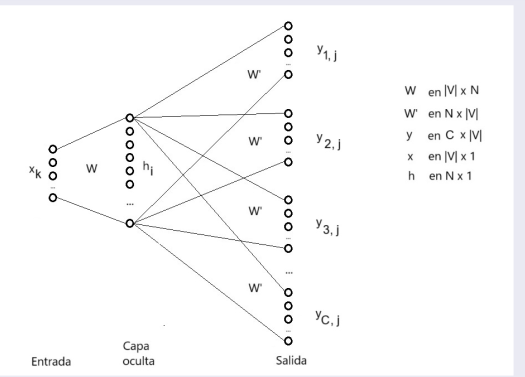
\includegraphics[width=0.6\textwidth]{Skip_arq.png}
	\vfill
\end{frame}

\begin{frame}[fragile]{2b.1.2 Skip-gram}
	\begin{block}{\textbf{Definición:} Skip-gram}
		\justifying
		\vspace{0.1cm}
		\textbf{Propósito:} Es un modelo de aprendizaje automático para aprender representaciones de palabras que capturan el significado de las palabras basadas en su contexto. La diferencia con CBOW es que la entrada de la red es una palabra y la salida intenta predecir su contexto.\\
		\vspace{0.1cm}
		\textbf{Principio:} Skip-gram utiliza una palabra central para predecir un contexto de C palabras.\\
		\vspace{0.1cm}
		\textbf{Contexto vs. Predicción:} A partir de una palabra central ($p_O$), el modelo intenta predecir las palabras de su contexto ($p_{I,1}, p_{I,2}, ..., p_{I,C}$).
	\end{block}    
\end{frame}

\begin{frame}[fragile]{2b.1.3 Skip-gram: Representación de la entrada}
	\begin{block}{\textbf{Entrada del modelo}}
		\justifying
		\textbf{Palabra central:} se representa como un vector one-hot $x \in \mathbb{R}^{|V|}$, 
		donde $|V|$ es el tamaño del vocabulario.\\
		\vspace{0.2cm}
		Ejemplo: si $|V|=10\,000$ y la palabra central ocupa la posición 22, 
		entonces $x$ tiene un 1 en la posición 22 y 0 en las demás.\\
		\vspace{0.2cm}
		\textbf{Matriz de pesos de las conexiones entre la entrada y la capa oculta:} 
		\[
		W \in \mathbb{R}^{|V| \times N}
		\]
		donde $N$ es la dimensión del espacio de las representaciones vectoriales (ej. $N=300$).
	\end{block}
\end{frame}

\begin{frame}[fragile]{2b.1.4 Skip-gram: Representación vectorial}
	\begin{block}{\textbf{Cálculo de la representación vectorial de la palabra $p_I$}}
		\justifying
		La capa oculta no tiene función de activación. 
		Se obtiene directamente la representación vectorial de la palabra central:
		\[
		h = W^T x = v_{p_I}, \quad h \in \mathbb{R}^N
		\]
		donde $v_{p_I}$ es la representación vectorial asociado a la palabra central $p_I$.\\
		\vspace{0.2cm}
		Dimensiones:
		\begin{itemize}
			\item $x \in \mathbb{R}^{|V|}$ (one-hot).
			\item $W \in \mathbb{R}^{|V| \times N}$.
			\item $h \in \mathbb{R}^N$ (representación vectorial asociado a la palabra $p_I$).
		\end{itemize}
	\end{block}
\end{frame}

\begin{frame}[fragile]{2b.1.5 Skip-gram: Salida y softmax}
	\begin{block}{\textbf{Cálculo de probabilidades}}
		\justifying
		Para cada palabra $j$ en el vocabulario, se calcula:
		\[
		u_j = (v'_j)^T h, \qquad u \in \mathbb{R}^{|V|}
		\]
		donde $v'_j$ es el vector de salida correspondiente a la palabra $j$, 
		y $W' \in \mathbb{R}^{N \times |V|}$ es la matriz de salida.\\
		\vspace{0.2cm}
		Luego se aplica softmax:
		\[
		y_j = \frac{\exp(u_j)}{\sum_{k=1}^{|V|} \exp(u_k)}
		\]
		obteniendo la probabilidad de que la palabra $j$ aparezca en el contexto de $p_I$.
	\end{block}
\end{frame}

\begin{frame}[fragile]{2b.1.6 Skip-gram: Función de pérdida}
	\begin{block}{\textbf{Pérdida logarítmica}}
		\justifying
		Dado un contexto de $C$ palabras alrededor de la palabra central $p_I$, 
		la función de pérdida se define como:
		\[
		E = - \sum_{c=1}^{C} \log P(p_{O_c} \mid p_I)
		\]
		donde $p_{O_c}$ son las palabras del contexto.\\
		\vspace{0.2cm}
	\end{block}
\end{frame}

\begin{frame}[fragile]{2b.1.7 Skip-gram: Actualización}
	\begin{block}{\textbf{Reglas de actualización}}
		\justifying
		Durante el entrenamiento, los vectores de entrada y salida se ajustan.\\
		\vspace{0.2cm}
		Para los vectores de salida:
		\[
		v'_j \leftarrow v'_j - \eta \, E_{Ij} \, h
		\]
		Para el vector de entrada de la palabra central:
		\[
		v_{p_I} \leftarrow v_{p_I} - \eta \, EH^T
		\]
		donde:
		\begin{itemize}
			\item $\eta$ es la tasa de aprendizaje.
			\item $E_{Ij}$ depende del error para cada palabra del contexto.
		\end{itemize}
	\end{block}
	
\end{frame}

\begin{frame}[fragile]{2b.1.8 Skip-gram: Implementacion completa en Python}
	
	\begin{block}{}
		\begin{lstlisting}[language=Python]
			def entrenar_skipgram(ruta_corpus, nombre_pc, epocas=1, eta=0.001, N=300, C=4, W1=None, W2=None, intervalo_guardado=50):
			
				corpus, vocab, vocab_size, word_to_idx, idx_to_word = cargar_corpus(ruta_corpus)
				W1, W2 = inicializar_pesos(vocab_size, N, W1, W2, cparray=True)
				indice_tuplas = generar_tuplas_central_contexto(corpus, word_to_idx, C)
				total_pares = len(indice_tuplas)
				
				print(f"Comienzo de entrenamiento con {epocas} epocas.")
				for epoca in range(epocas):
					for i, (i_central, i_contextos) in enumerate(indice_tuplas):              
		\end{lstlisting}
	\end{block}
\end{frame}

\begin{frame}[fragile]{2b.1.9 Skip-gram: Implementacion completa en Python}
	
	\begin{block}{}
		\begin{lstlisting}[language=Python]
			# ---Propagacion---
			h = W1[i_central].reshape(-1, 1)
			u = W2.T @ h
			y = softmax_cp(u)
			
			# ---Retropropagacion---
			EI = y.copy()
			EI[i_contextos] -= 1
			W2 -= eta * (h @ EI.T)
			
			EH = W2 @ EI
			W1[i_central] -= eta * EH.T[0]
			
			if i % 1000 == 0:
			print(f"Epoca {epoca}, Par: {i}/{total_pares}")
			
			print(f"Fin de epoca: {epoca}")                
		\end{lstlisting}
	\end{block}
\end{frame}

\begin{frame}[fragile]{2b.1.10 Skip-gram: Implementacion completa en Python}
	
	\begin{block}{}
		\begin{lstlisting}[language=Python]
			# ---Guardado de Pesos---
			if epoca % intervalo_guardado == 0 or epoca == epocas - 1:
			nombre_archivo = f'pesos_skipgram_{nombre_pc}_epoca{epoca}.npz'
			guardar_modelo(nombre_archivo, W1, W2, eta=eta, N=N, C=C, cparray=True)
			
			print(f"Entrenamiento con {epocas} terminado.")
			return W1, W2                
		\end{lstlisting}
	\end{block}
\end{frame}

\begin{frame}[fragile]{2b.1.11 Skip-gram: Propagación hacia adelante}
	\begin{block}{\textbf{Fórmulas}}
		\[
		h = W^T x = v_{p_I}, \quad
		u = W'^T h, \quad
		y = \text{softmax}(u)
		\]
	\end{block}
	
	\begin{block}{\textbf{Implementación en Python}}
		\begin{lstlisting}[language=Python]
			#   Propagacion  
			h = W1[i_central].reshape(-1, 1)   
			u = W2.T @ h                        
			y = softmax_cp(u)                 
		\end{lstlisting}
	\end{block}
\end{frame}

\begin{frame}[fragile]{2b.1.12 Skip-gram: Cálculo del error}
	\begin{block}{\textbf{Pérdida}}
		\[
		EI = y - t
		\]
		donde $t$ es el vector one-hot con 1 en la posición de la palabra de contexto.
	\end{block}
	
	\begin{block}{\textbf{Implementación en Python}}
		\begin{lstlisting}[language=Python]
			# Retropropagacion 
			EI = y.copy()
			EI[i_contextos] -= 1   # resta 1 en las posiciones del contexto
		\end{lstlisting}
	\end{block}
\end{frame}

\begin{frame}[fragile]{2b.1.13 Skip-gram: Actualización de $W'$}
	\begin{block}{\textbf{Regla de actualización}}
		\[
		v'_j \leftarrow v'_j - \eta \, E_{Ij} \, h
		\]
	\end{block}
	
	\begin{block}{\textbf{Implementación en Python}}
		\begin{lstlisting}[language=Python]
			# Actualizacion de la matriz de salida W2
			W2 -= eta * (h @ EI.T)
		\end{lstlisting}
	\end{block}
\end{frame}

\begin{frame}[fragile]{2b.1.14 Skip-gram: Actualización de $W$}
	\begin{block}{\textbf{Regla de actualización}}
		\[
		v_{p_I} \leftarrow v_{p_I} - \eta \, EH^T, 
		\quad \text{donde } EH = W' EI
		\]
	\end{block}
	
	\begin{block}{\textbf{Implementación en Python}}
		\begin{lstlisting}[language=Python]
			EH = W2 @ EI
			W1[i_central] -= eta * EH.T[0]
		\end{lstlisting}
	\end{block}
\end{frame}
	
\section{Ejercicio 2b: negative sampling}

\begin{frame}{}
	\centering
	\Large Skip-gram (Negative Sampling)\\
	\vspace{0.8cm}
	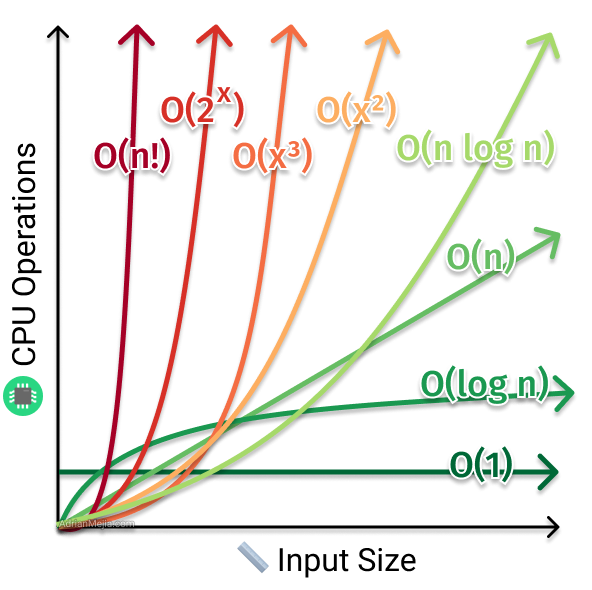
\includegraphics[width=0.5\textwidth]{big-o}
\end{frame}

\begin{frame}[fragile]{2b.2.1 Skip-gram(NS)}
	\begin{block}{\textbf{Definición:} Skip-gram con muestreo de ejemplos negativos (Negative Sampling)}
		\justifying
		\vspace{0.1cm}
		\textbf{Propósito:} Reducir el costo computacional al actualizar los pesos en el modelo SkipGram.\\
		\vspace{0.1cm}
		\textbf{Principio:} Actualizar a W' aplicando la técnica de muestro de ejemplos negativos mencionada anteriormente\\
	\end{block}
\end{frame}

\begin{frame}{2b.2.2 Lógica de álgoritmo}
	\begin{block}{\textbf{Función:} entrenar\_skipgram\_neg\_samp()}
		Al ejecutarse:
		\begin{itemize}
			\item Se carga el corpus y vocabulario
			\item Se inicializan los pesos $W$ y $W'$.
			\item Se generan las tuplas $(\text{central}, \text{positivos}, \text{negativos})$.
			\[
			\begin{array}{ccccc}
				\textcolor{red}{\underbrace{\text{encontraría}\quad \text{a}}_{\text{negativos}}} &
				\textcolor{green}{\underbrace{\text{la}\quad \text{maga}}_{\text{positivos}}} &
				\textcolor{blue}{\underbrace{\text{?}}_{\text{central}}} &
				\textcolor{green}{\underbrace{\text{tantas}\quad \text{veces}}_{\text{positivos}}} &
				\textcolor{red}{\underbrace{\text{me}\quad \text{había}}_{\text{negativos}}}
			\end{array}
			\]
			\item Se \textbf{entrenan} los pesos por $q$ épocas y por cada tupla generada.
			\item se guardan los pesos cada $p$ épocas.
		\end{itemize}
	\end{block}
	
\end{frame}

\begin{frame}[fragile]{2b.2.3 Código de bucle de entrenamiento}
	\justifying
	\begin{lstlisting}[language=Python]
for epoca in range(epocas):
	for i, (i_central, i_positivos, i_negativos) in enumerate(
		indice_tuplas):
		i_total = i_positivos + i_negativos
		
		h = W1[i_central].reshape(-1, 1)
		u = W2[:, i_total].T @ h
		y = sigmoide_np(u)
		
		EI = y.copy()
		EI[:len(i_positivos)] -= 1
		W2[:, i_total] -= eta * (h @ EI.T)
		
		EH = W2[:, i_total] @ EI
		W1[i_central] -= eta * EH.T[0]
	\end{lstlisting}
\end{frame}


\begin{frame}[fragile]{2b.2.5 Dificultades}
	\justifying
	\begin{block}{}
		La función \texttt{sigmoide\_np} generaba valores \textbf{NaN} en las matrices de pesos $W$ y $W'$ al actualizarlos.
	\end{block}
	
	\begin{lstlisting}[language=Python]
def sigmoide_np(x):
	return 1 / (1 + np.exp(-x))
	\end{lstlisting}
	
	\begin{block}{}
		Para solucionar esto utilizamos un valor de $\eta$ menor (0,001).
	\end{block}
	
\end{frame}

\begin{frame}{2b.2.6 Resultados}
	...
\end{frame}

\end{document}